\section{Experiments and Results}
\label{sec:results}

% MSB - what ground truth?  This is confusing, what do you mean by ground truth?
All our experiments have been completed with the inexpensive consumer
quadcopter called a Parrot's AR Drone 2.0. We have used the ROS based
ARDrone Autonomy Driver to communicate with the drone. For the purpose
of showing the efficacy of this paper, we also took a picture of the
scene from a distance with a 5 mega-pixel camera to better understand
the scene.

We have implemented our algorithm in C++ using the OpenCV library
(OpenCV 2.4.9). Experiments were performed on a PC with Intel Core i7
processor(@3.4GHz) and 8GB RAM.  The source code to produce
interesting images from a video, and to generate the super-panorama,
as well as the data sets used in this paper will be made publicly
available.

\subsection{Selecting Images}

In our first experiment, we wanted to ensure that the selection of
images done was comprehensive and useful.  We sent the drone to image 
an outdoor scene with no vacant space. This experiment was conducted
in an outdoor environment. We note here that there were approximately
3000 images in the raw video.  Autostitch was unable to cope  when fed
with this large number of frames.

One way to produce some sort of mosaic was to simply reduce the amount
of data given to Autostitch.  Figure~\ref{fig:sac3}(a) shows uniformly
(time) sampled images from the video.  When these sampled images are
given to Autostitch or to Adobe Photoshop, we find
(Figure~\ref{fig:sac3}(b)) that these programs are able to produce
some output, but the results are not satisfactory.

% MSB - no details to the saliency selection algorithm.
Instead of feeding time-sampled images, we ran our saliency selection
algorithm (as explained in Section~\ref{sec:selection}) on the video
which resulted in $N = 5$ images.  Though the number of input images
in the video is large, the total distance covered by the quadcopter in
this duration (of around 90 seconds) is small; thus the
number of distinct images returned by the algorithm shows a dramatic
reduction. Figure~\ref{fig:sac3}(c) shows examples of selected images.
Many of the images are similar to the time sampled version; however,
the occasional differences are enough to make Autostitch work. The
results are shown in Figure~\ref{fig:sac3}(d).


\begin{figure*}[h!]
\centering
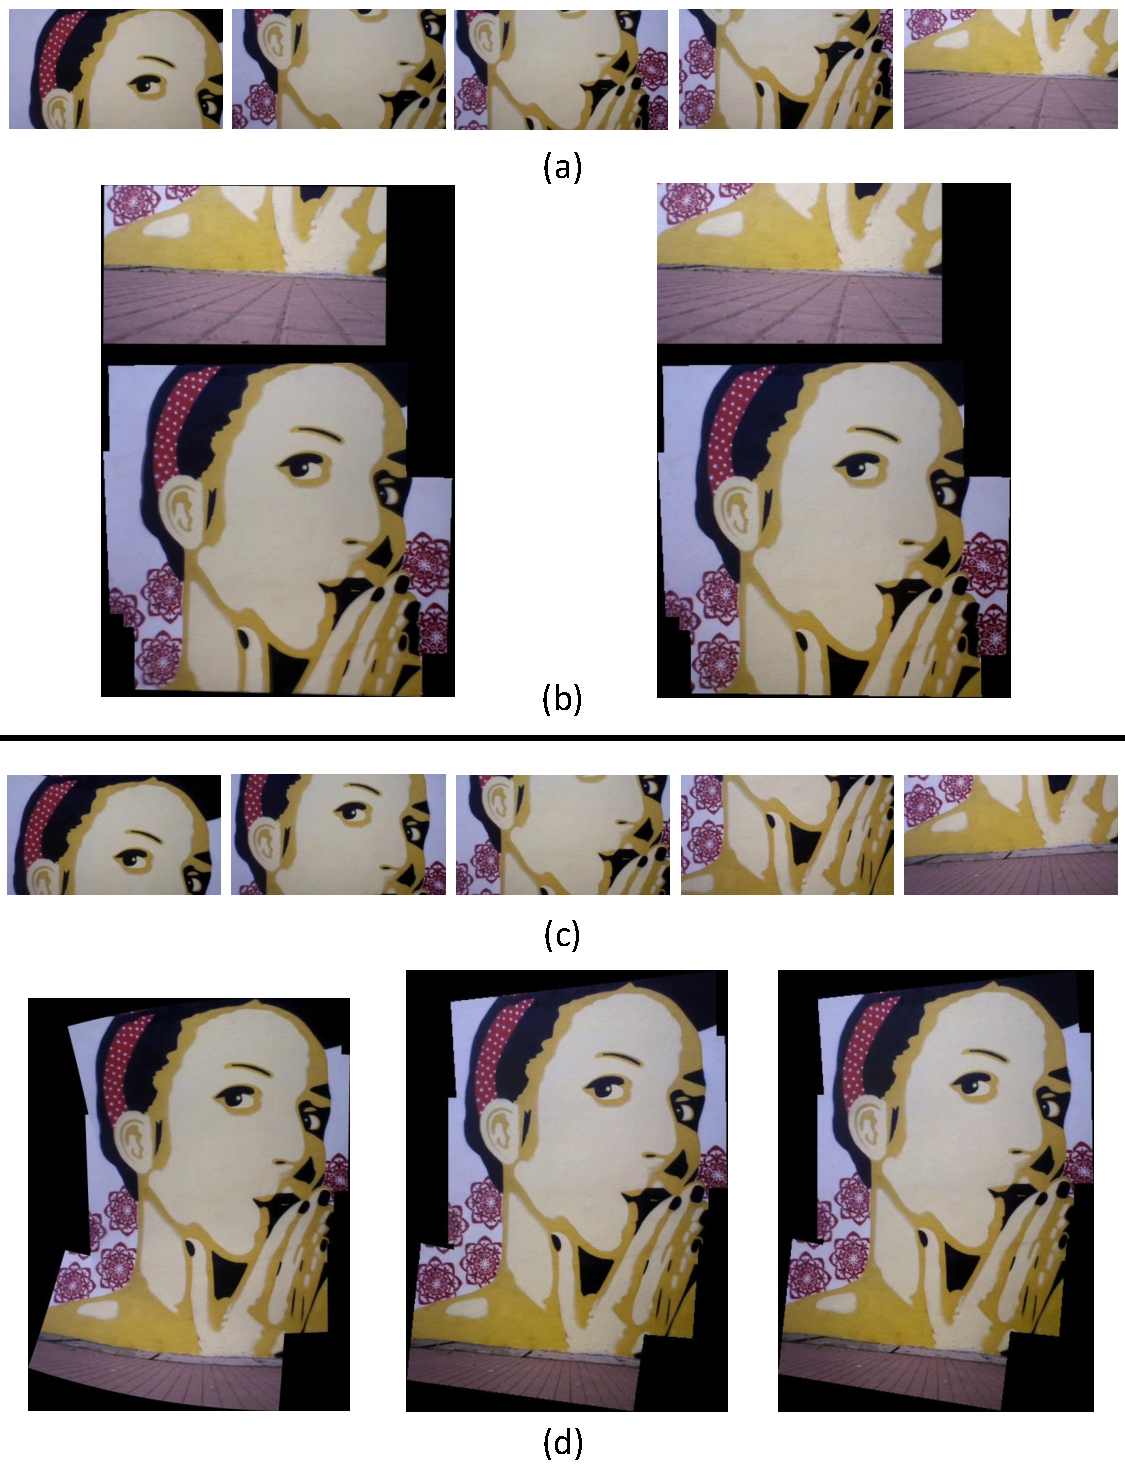
\includegraphics[width=0.87\linewidth]{figures/ValidationResult}
\caption{ (a) Uniformly sampled images from an outdoor video
  expedition.  (b) Output of the state of the art photo stitchers
  (left:Autostitch, right:Adobe Photoshop PS6) on uniformly time
  sampled images.  As time sampled images do not guarantee coverage of
  the scene, the panorama is broken. The top portions do not belong at
  the right place (see (d) (c) Salient image selection from the set of
  approximately 9000 images using positional information. (d) When
  salient images are given to Autostich (left) and Photoshop (middle),
  we can create a panoramic mosaic (since there are no vacant
  spaces). We also show the results from our stitching algorithm
  (bottom right).}
\label{fig:sac3}
\end{figure*}

In summary, this experiment provides evidence to show that (a) our
saliency selection algorithm is reasonable and (b) our stitching
results are comparable to that of Autostitch for the kind of scenes
considered.

\subsection{Indoor Imagery with Vacant Spaces}

% MSB - again, no details to the selection algorithm, so the reader will
% have no idea how you came up to $N=4$.
Our next selection of experiments were conducted in an indoor
environment.  The input stream had about 4300
images. The selection algorithm (Section~\ref{sec:selection}) pruned the video
into $N=4$ images.
A sample of the selected images are seen in Figure~\ref{fig:teaser}.

\begin{figure*}[h!]
\centering
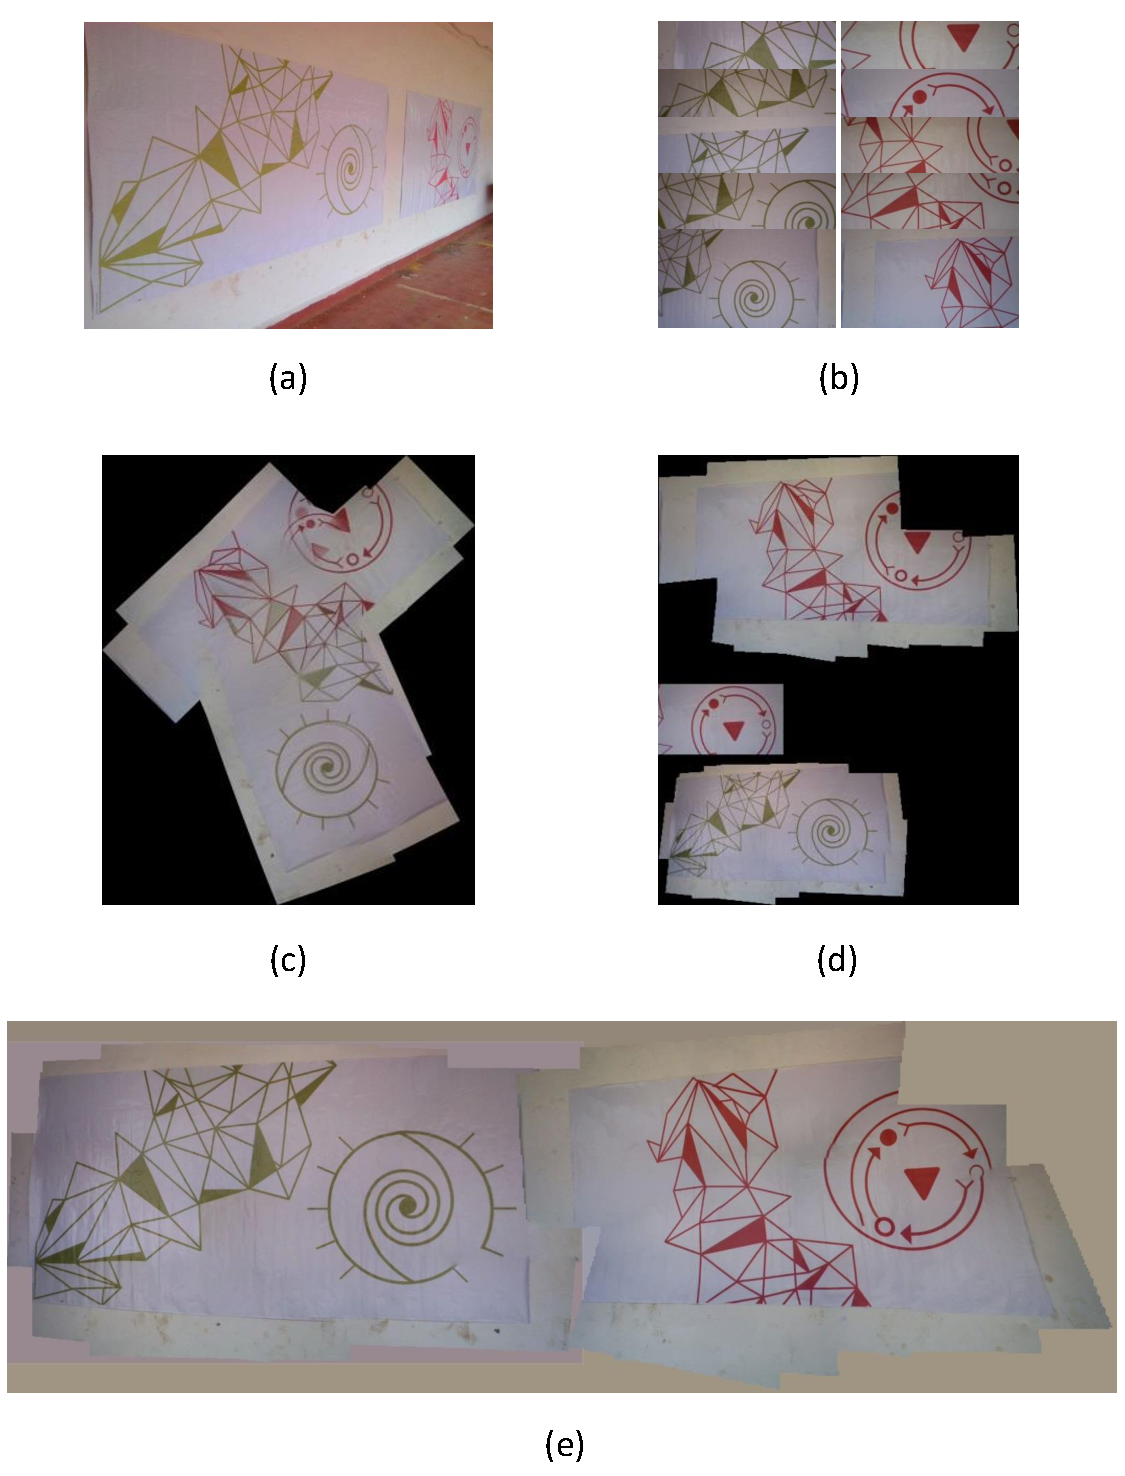
\includegraphics[width=0.86\linewidth]{figures/results}
\caption{(a) An outdoor scene captured by a standard camera in an
  exhibition. The approach to the area is normally cordoned off and one
  needs permission to get a quadcopter to take the picture.  Notice a
  significant gap between the two posters.  (b) Pruned images from the
  quadcopter video using our saliency algorithm. (c) Output of
  Autostitch on the selected images. The mosaic is not reasonable
  presumably because of the confusion in features. (d) Output of Adobe
  Photoshop PS6 on the selected images. The vacant space posed a
  problem to the feature matching algorithm, so instead of a mosaic,
  individual pieces were output as mini-panoramas (e) Our output on
  the selected images. We are able to join two posters (separated by
  vacant space) using IMU data.}
\label{fig:results}
\end{figure*}

There were two disconnected components in the resulting graph.
Autostitch was unable to produce any reasonable output as seen in
Figure~\ref{fig:teaser}.  The scene, captured from a distance is also
shown.  One can see a better orthographic view of the posters.

\subsection{Outdoor Imagery with Vacant Space}
Our next set of experiments were conducted in an outdoor
environment. The input stream had about 12000 images. The selection
algorithm pruned the video into $N=30$ images. A sample of the
selected images are seen in Figure~\ref{fig:results}.  The scene as
captured by a smartphone can also be seen, as well as the comparison
of outputs of state of the art stitchers with output of our
algorithm. Figure~\ref{fig:results} shows the comparison of outputs of
state of the art stitchers with the output of our algorithm.

% Figure \ref{fig:results2} shows comparison of outputs of state of the art
% stitchers with output of our algorithm on another dataset.

% \begin{figure}[h!]
% \centering
% 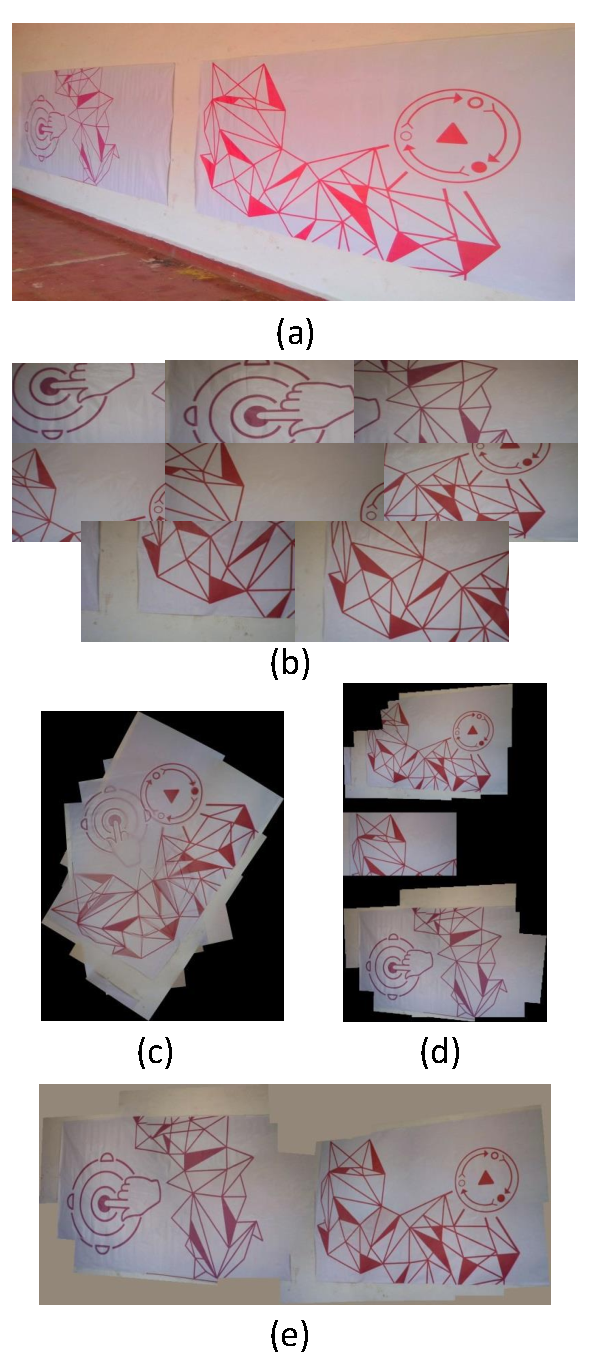
\includegraphics[width=0.8\linewidth]{figures/Purple_red}
% \caption{(a) Another outdoor scene captured by a standard camera in an
%   exhibition. The approach to the area is normally cordoned off and one
%   needs permission to get a quadcopter to take the picture.  Notice a
%   significant gap between the two posters.  (b) Pruned images from the
%   quadcopter video using our saliency algorithm. (c) Output of
%   Autostitch on the selected images. The mosaic is not reasonable
%   presumably because of the confusion in features. (d) Output of Adobe
%   Photoshop PS6 on the selected images. The vacant space posed a
%   problem to the feature matching algorithm, so instead of a mosaic,
%   individual pieces were output as mini-panoramas (e) Our output on
%   the selected images. We are able to join two posters (separated by
%   vacant space) using IMU data.}
% \label{fig:results2}
% \end{figure}

Please see supplementary material for results on other datasets.
